\documentclass{article}
\usepackage[margin=2cm]{geometry}
\usepackage{graphicx}
\usepackage{hyperref}
\hypersetup{
    colorlinks=true,
    linkcolor=blue,
    filecolor=magenta,      
    urlcolor=cyan,
}

\begin{document}
\title{{\Huge Net Computing} \\[.5cm] {\Large Nodes Measurement System}}
\author{
\begin{tabular}{r l}
	Martijn Luinstra & s\,2199289 \\
	Emilio Oldenziel & s\,2509679 \\
	Yannick Stoffers & s\,2372061
\end{tabular}
}

\maketitle

\section{Introduction}
    % What our application does %
    We created an nodes measurement system where a user can monitor nodes (or any other machine) in a network.
    

\newpage
\section{Architecture}
    % Overview of how the system is set-up %
    The system consists of a central server, nodes that are measured and clients that are connected to the central server with their browser. The nodes send their measurements to the central server using message queueing, the central server has a worker that handles the message queue and takes the measurement from the queue and than processes them. The worker saves the measurement in a database for archiving purposes and sends the measurement directly to the client's browser using the browser's websocket. More nodes that have to be measured can be added by using web services, the node asks the central server if he can be monitored, if that is possible, the central server gives setup data to the node like what its id is and where he has to queue his measurements.
    
    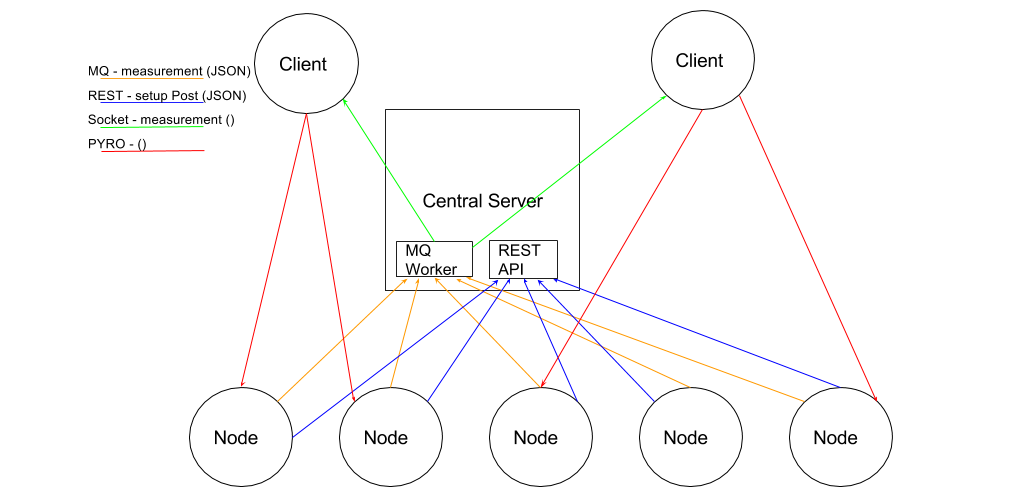
\includegraphics[scale=0.45]{architecture.png}

\section{Design choices}
    %explain why we used one central server with workers instead of p2p
    We chose to have a centralised server so that we have one point that does the 'bookkeeping' of which nodes are monitored, but also to make it simpler that nodes and client connect to the same point.
    
    %Why we chose python
    The language that we used for this project is Python, we chose that because we all a lot more experience with Python than with Java. For projects like this where we have to show that we understand the concepts and techniques Python is nicer because we don't have to deal with the generics of Java and can concentrate more on the main concepts. Speed is not an issue in this system because Python is fast enough to handle all the operations without human noticeable latency.
    
    % explain why we used JSON %
    We used JSON as datatype for our communication, mainly because it is very simple to use in python. There is a standard JSON library in python that can create a JSON object from a dictionary (python version of a HashMap) and vice versa.
    In this way we could serialize our data in a simple way and then send it.
    JSON is nowadays the most used data-type for sending object over the internet because of its simplicity and readability. %vague remark%
    
\section{Application Flow}
    First the central server and its workers are started. A node can ask the server if he can be observed and gives his name and ip-address, the server responds with No or gives the setup data. If the node received the setup data the node will start a worker thread that does measurements from the hardware and queues this to the message queue of the central worker, the node will continue doing this every second till the thread is stopped. The central server's message queue worker will save the measurement and send it directly to all connected browsers. If a node has a major difference in some metric (e.g. the CPU temperature will increase very rapidly) this will be seen on the dashboard on the browser. % How to do PYRO Stuff %
    

\section{Techniques}
    %Flask (API, Server, Models, sockets), RabbitMQ(Pika), PYRO
    We made use of multiple frameworks for this project. For the central server we used \href{http://flask.pocoo.org/}{Flask} with the \href{https://flask-restful.readthedocs.io/en/0.3.5/}{Flask-Restful} API to do the initial setup of a node, this API uses REST to handle requests. As server for the API we used the development server of Flask, this is a lightweight server that has everything to demonstrate the application. To store the measurements \href{http://flask-sqlalchemy.pocoo.org/2.1/}{Flask SQL-alchemy} is used with an SQLite database for simple storage of data from the demo.
    For Message queueing RabbitMQ is used, to use RabbitMQ with python we used \href{https://github.com/pika/pika}{pika} which is a Python interface to RabbitMQ. 


\end{document}